
% This LaTeX was auto-generated from MATLAB code.
% To make changes, update the MATLAB code and republish this document.

\documentclass{article}
\usepackage{graphicx}
\usepackage{color}

\sloppy
\definecolor{lightgray}{gray}{0.5}
\setlength{\parindent}{0pt}

\begin{document}

    
    
\subsection*{Contents}

\begin{itemize}
\setlength{\itemsep}{-1ex}
   \item Unknown Input Observer Dynamic System Matricies
   \item Construct the state space system
   \item Step one: Check rank
   \item Step two: Compute Observer Matricies
   \item Step three: check observability
   \item Pole Placement
   \item Finish observer design
   \item Simulation results
   \item Sim the system
   \item Plot the results
\end{itemize}


\subsection*{Unknown Input Observer Dynamic System Matricies}

\begin{par}
This example is form the book: Robust Model Based Fault Diagnosis for Dynamic Systems by J. Chen Please see the associated ShareLaTeX pdf file "UIO and Examples"
\end{par} \vspace{1em}
\begin{verbatim}
A = [-1 1 0;-1 0 0;0 -1 -1];
B = [-1;0;0];
C = [1 0 0;0 0 1];
D = 0;
E = B;
\end{verbatim}


\subsection*{Construct the state space system}

\begin{par}
Let us construct the system as a state space object for simulation.
\end{par} \vspace{1em}
\begin{verbatim}
sys = ss(A,B,C,D);
\end{verbatim}


\subsection*{Step one: Check rank}

\begin{par}
We check to see if the rank(CE) = rank(E) = 1
\end{par} \vspace{1em}
\begin{verbatim}
rank(C*E)
rank(E)
\end{verbatim}

        \color{lightgray} \begin{verbatim}
ans =

     1


ans =

     1

\end{verbatim} \color{black}
    

\subsection*{Step two: Compute Observer Matricies}

\begin{par}
Since we have no issues in the previous step, let us compute the observer matrices now:
\end{par} \vspace{1em}
\begin{verbatim}
H = E*inv((C*E)'*(C*E))*(C*E)'
T = eye(3)-H*C
A1 = T*A
\end{verbatim}

        \color{lightgray} \begin{verbatim}
H =

     1     0
     0     0
     0     0


T =

     0     0     0
     0     1     0
     0     0     1


A1 =

     0     0     0
    -1     0     0
     0    -1    -1

\end{verbatim} \color{black}
    

\subsection*{Step three: check observability}

\begin{par}
We must check the system A1,C observability
\end{par} \vspace{1em}
\begin{verbatim}
rank(obsv(A1,C))
\end{verbatim}

        \color{lightgray} \begin{verbatim}
ans =

     3

\end{verbatim} \color{black}
    

\subsection*{Pole Placement}

\begin{par}
Pole placement is used to assign the observer poles
\end{par} \vspace{1em}
\begin{verbatim}
K1 = place(A',C',[-2,-10,-5])'
\end{verbatim}

        \color{lightgray} \begin{verbatim}
K1 =

    6.7231   -3.7816
    7.5581  -11.3458
   -3.0543    8.2769

\end{verbatim} \color{black}
    

\subsection*{Finish observer design}

\begin{par}
Finally, the F and K matricies are computed
\end{par} \vspace{1em}
\begin{verbatim}
F = A1-K1*C
K = K1 + F*H
\end{verbatim}

        \color{lightgray} \begin{verbatim}
F =

   -6.7231         0    3.7816
   -8.5581         0   11.3458
    3.0543   -1.0000   -9.2769


K =

         0   -3.7816
   -1.0000  -11.3458
         0    8.2769

\end{verbatim} \color{black}
    

\subsection*{Simulation results}

\begin{par}
Set up simulation initial condiditons
\end{par} \vspace{1em}
\begin{verbatim}
x1_0 = 100;
x2_0 = -100;
x3_0 = 1;

d = 10;
\end{verbatim}


\subsection*{Sim the system}

\begin{verbatim}
sim('exOne')
\end{verbatim}

        \color{lightgray} \begin{verbatim}Warning: Input port 3 of 'exOne/UIO/z' is not connected. 
Warning: Output port 1 of 'exOne/UIO/z/u' is not connected. 
Warning: Using a default value of 0.2 for maximum step size.  The simulation
step size will be equal to or less than this value.  You can disable this
diagnostic by setting 'Automatic solver parameter selection' diagnostic to
'none' in the Diagnostics page of the configuration parameters dialog 
\end{verbatim} \color{black}
    

\subsection*{Plot the results}

\begin{verbatim}
t = linspace(1,10,length(X_hat));
figure(1),plot(t,X),hold on
plot(t,X_hat(:,1),'xb'),hold on
plot(t,X_hat(:,2),'xg'),hold on
plot(t,X_hat(:,3),'xr')
xlabel('Time in seconds'),ylabel('State trajectory and estimate')
title('Dynamic system state and UIO estimate')
legend('x_1','x_2','x_3','x_1 hat','x_2 hat','x_3 hat')
\end{verbatim}

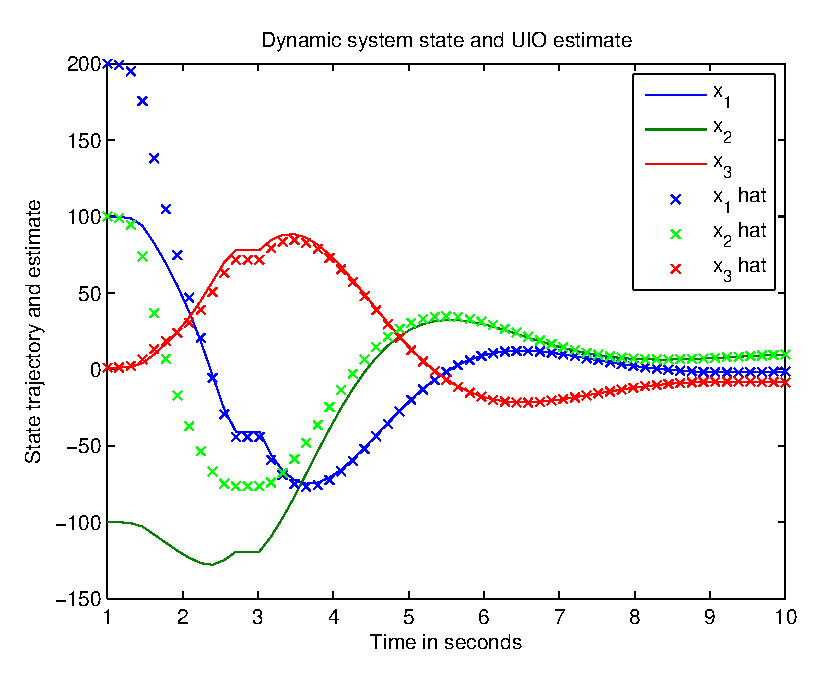
\includegraphics [width=4in]{bookEx_01.eps}



\end{document}
    
